\chapter{Mapping Species-Specific Ionization in Warm Dense Crystalline MgO Under Extreme X-ray Heating }
\label{mgo}

Oliver Hoidn, Ryan Valenza, Gerald T.
Seidler\textsuperscript{(*)}\textsubscript{,} Alexander Ditter, William
Holden, Evan Jahrman, Luis Avila, Galen O'Neil, Josh Kas, Fer Vila, and Sam Vinko.

Physics Department, University of Washington, Seattle WA

National Institute of Standards and Technology, Boulder CO

(*) seidler@uw.edu

We report a study of the x-ray diffraction of nanocrystalline MgO during
heating by high-intensity x-ray pulses from an x-ray free electron laser
(XFEL). Careful consideration of the three lowest Miller index Bragg
peaks gives strong evidence that the MgO remains crystalline during the
XFEL pulses and also that there is a disproportionate ionization of the
O\textsuperscript{2-} ion at surprisingly low incident flux densities
with respect to what would naively be expected from the unperturbed
crystalline ground-state electronic properties. We tentatively attribute
this to the likely introduction of a significant density of states into
the MgO ground-state energy gap as a consequence of high site disorder
of the charge state of the Mg and O ions. The full dependence of the
nominal ionization difference between the two crystallographic sites
shows a plateau at intermediate incident flux and a final rise at our
highest incident flux densities. These results are compared and
contrasted with theory.  This study emphasizes
the value of wide-angle x-ray diffraction coupled with the choice of
model systems for x-ray heating where the unit cell has sufficient
complexity that the Bragg peaks have widely different degrees of
constructive or destructive interference between the different sites in
the unit cell. We discuss possible future directions, including the use
of x-ray pump / x-ray probe XFEL studies of warm, dense crystalline
matter as a way to interrogate, under conditions better approaching
local thermodynamic equilibrium of electronic degrees of freedom, the
electronic structure at intermediate degeneracies where theoretical
treatment remains a topic of ongoing research.

In preparation, Phys. Rev. B (?) \textbf{\\}

\section{Introduction}

The `warm dense matter' (WDM) regime resides in an important and
theoretically interesting middle-ground between conditions typical of
high-pressure studies in condensed matter physics and those instead of
great interest to contemporary plasma physics, where atoms are fully
ionized. WDM is defined by partial ionization, solid-like or higher
densities, substantial Fermi degeneracy (\(T \leq \ E_{F}\)), and values
for the plasma coupling parameter Γ of order unity or larger. (cite
doi:10.1088/0741-3335/47/12B/S31 and others). Beyond intrinsic interest
in understanding this exotic physical regime, the collective properties
of WDM---such as its equations of state (EOS), opacities, and
viscosities---are of fundamental importance in geophysics, planetary and
stellar astrophysics, and inertial confinement fusion (ICF). (cites)
Validating models of WDM requires pushing existing analytical and
\emph{ab initio} theoretical frameworks beyond their
presently-demonstrated ranges of applicability. The bootstrapping of WDM
models thus demands good empirical constraints.

WDM, however, presents unique practical challenges. While some obvious
difficulties accrue from the details of how this transient state of
matter is actually created, hard problems arise from the question of
experimental diagnostics. Specifically, the high opacity of dense,
partially-ionized matter renders ineffective the well-developed suite of
optical-wavelength tools that are regularly used to obtain detailed
microscopic information for low density plasmas. The community has
therefore turned to x-ray wavelength diagnostics, each of which has a
different connection to microscopic observables of interest. X-ray
absorption spectroscopy interrogates the unoccupied electronic density
of states, x-ray fluorescence informs us about semi-core and core-level
occupancies of the ions, and elastic and inelastic x-ray scattering
characterize the real-space charge density and momentum-space
distribution functions, respectively.

The role of elastic x-ray scattering, i.e., x-ray diffraction (XRD), in
the study of crystalline WDM has recently been discussed by Valenza and
Seidler {[}cite{]}. While all early XRD studies of WDM were performed in
laser-shock studies where long-range crystalline order of the target is
destroyed, those authors instead address the question of WDM created by
heating of crystalline targets by the extremely fast pulses created by
x-ray free electron lasers (XFELs). While one key result of that work is
the large contribution to XRD of the nominally `free' electrons for
low-Z systems, there are two overarching perspectives in that work that
help motivate the present study. First, XRD from crystalline WDM
provides an important testing ground for finite-T electronic structure
theory, giving direct measurement of the fundamental quantity predicted
in DFT approaches, i.e., the spatial distribution of charge density. For
example, for low-Z systems, finite-T studies of XRD might be used to
give an especially salient inquiry into exchange functional effects
under intermediate degeneracy of the unbound electrons. Second, and of
greater relevance here, XRD from a WDM state where the ion cores are at
least effectively stationary is a rich experiment that, through the
careful choice of target material crystal structure, can be designed to
have far higher information content about microscopic parameters, such
as species-specific ionization states, than has been the case in studies
of disordered WDM.

We report here a study of the XRD from nanophase XFEL-heated targets of
the simple compound MgO. In the context of the above discussion, this
choice is highly desirable. First, MgO, which has the NaCl rock-salt
structure, is an example of the simplest crystal structure where there
are low-angle Bragg peaks that have either purely constructive or purely
destructive interference between the dissimilar species in the unit
cell. This property is nontrivial, and it gives the experiment
sensitivity to not just the average ionization across the unit cell but
instead the ionization of each species. Second, the combination of
slightly heavier atoms than in the Valenza {[}cite{]} work together with
favorably distributed conduction-band charge densities allows
interpretation in the context of a simple atomic form factor model that
ignores the contributions to XRD from the unbound electrons. Third, the
long semicore lifetime of Mg 2p holes provides an interesting problem
for the present work, where there is then a meaningful competition
between O valence-level and Mg 2p-level depopulation, but also provides
a natural extension to the future where variable-delay x-ray pump/probe
studies will be able to measure systems' responses to long-lived
electronic excitations with fine time resolution compared to durations
of the nonequilibrium states involved. Finally, while the nanophase
nature of the target poses some added complications in calculating the
average energy actually deposited in each unit cell, it ensures good
sample isotropy so that the XRD rings are uniform for each single shot.
This averts a problem that can arise in coarse-grained powder
diffraction samples, wherein a relatively small number of crystallites
in the probed sample volume results in insufficient sampling of the
distribution of random crystallite orientations.

We find no signatures of long-range lattice disorder, such as
Deybe-Waller or `Bragg gating' effects, across a range of energy
deposition densities reaching 150 eV per unit cell. However, we measure
a monotonic rise in intensity of the 111 peak of MgO with increasing
XFEL flux density; we conclude that this anomalous effect results from a
loss of destructive interference within the MgO unit cell as the valence
electrons of O progressively delocalize. This is an observation of
short-range, purely electronic charge reorganization in a solid-density
plasma that constitutes an initial demonstration of the type of effect
predicted by Valenza et al. (cite). Although we find that the MgO
system's lack of local thermal equilibrium (LTE) limits the utility of
comparisons to theory, the experiment validates wide-angle XRD as an
effective probe of local real-space electronic reorganization in warm
dense matter. It thus presents the appealing prospect of future XRD
studies on XFEL-heated WDM and solid-density plasmas designed to
empirically constrain DFT-based predictions of finite-temperature
electronic structure.

The manuscript continues as follows. First, in section II we describe
the experimental configuration, data reduction procedure, and several
modeling approaches used to interpret the data. These include the use of
the collisional radiative code SCFLY to model the time-evolution of
charge state populations at high energy densities; finite-temperature
DFT simulations in VASP to establish comparison between the low-energy
density experimental regime and a LTE-based model; and two \emph{ad-hoc}
models of O valence-level ionization. In section III we present
experimental and modeling results, and in section IV we conclude.

\section{II. Methods}

\subsection{II. A. Experimental Details}

The experiment was performed at the matter of extreme conditions (MEC)
endstation of the Linac Coherent Light Source (LCLS), where XFEL pulses
were used to excite MgO samples consisting of a 100 nm-thick layer of
PMMA with embedded MgO nanoparticles (Sigma Aldrich, typical size 50 nm)
on an 8 um-thick polyimide substrate. We used self-amplified stimulated
emission (SASE) pulses of 45 fs mean duration, average pulse energies of
2 mJ (check this), and a nominal x-ray energy of 9 keV. Variations in
the mean photon energy of each pulse are monitored by a downstream
dispersive spectrometer. We controlled flux density incident on the
sample via a stack of Be lenses, with which we varied the focal spot
diameter of XFEL pulses at the sample position from 2 to 60 um; these
diameters were determined using an ablative imprint method to measure
the spatial profile of the focused XFEL beam (cite
\url{http://doi.org/10.1016/j.nima.2010.12.040}). Using the full
available range of focal spot sizes and a constant (unattenuated) beam
intensity, we obtained incident flux densities ranging from 30 to 2000
J/cm\textsuperscript{2}.

During data collection the sample's position was rastered at a rate of
100 um between the XFEL pulses, whose repetition
rate was 120 Hz. At every XFEL pulse the Bragg scattering signal was
collected and read out from a quad CSPAD solid state detector having 800
x 800 resolution and a pixel pitch of 100 um. (cite CSPAD papers) The 8
x 8 cm\textsuperscript{2} active area of the detector subtended the
range of scattering angles from 10 to 58 degrees, encompassing the 111,
200, and 220 Bragg reflections of MgO (located at 33.5, 38.8, and 55.9
degrees, respectively).

\subsection{II.B. Data Reduction and Analysis}

Several steps of processing and event selection were performed prior to
generating powder diffraction patterns. For each event the quad CSPAD
readout was corrected by subtracting pixel pedestals (measured using
previously-collected dark exposures) as well common-mode noise in each
of the detector's 16 individual tiles. (cite CSPAD paper). Due to the
small number of photon hits in a single shot residual ADC noise often
dominated the Bragg scattering signal. To address this we made use of a
standard component of the analysis pipeline for CSPAD data in low-photon
count rate experiments at the LCLS, such as macromolecular imaging and
crystallography, which identifies clusters of spatially-concentrated
signal resulting from x-ray photon hits, rejecting the output of
noise-dominated pixels.

For each LCLS pulse a powder diffraction pattern is generated from the
quad CSPAD frame by the summation of elliptically-shaped strips of
pixels at equal scattering angle. The mapping of pixel coordinate to
scattering angle is calculated from the CSPAD's location and orientation
relative to the sample and incident XFEL beam; this geometry is in turn
obtained from the conic section parameters of powder diffraction peaks
in data from a known reference material measured in the same
source-detector geometry. After generation of a powder pattern, two
corrections are made. First, the each peak is shifted to correct for
angular offsets caused by imperfect flatness of the sample substrate and
also event-to-event jitter in the mean photon energy of the XFEL.
Second, a linear fit is made to the background of each peak, and this
background is subtracted from the peak signal. The signal-to-background
ratio for this peak is then computed by comparison of the background
level derived from the linear fit to a simple integration of the
background-subtracted peak. Events in which any of the peak
signal-to-background ratios fall below a threshold (chosen to be 0.2)
are rejected in subsequent summation over data from multiple events.

Bragg peak scattering intensity is the most significant derived quantity
from each powder pattern in this study, but its estimation requires
correcting the effect of variations in the total scattering signal
caused by sample non-uniformity and temporal variation of the XFEL pulse
energy. The latter contribution can be corrected using direct
measurement of incident pulse intensities available from an upstream
nitrogen detector; for comparison of Bragg peak intensities at different
flux density values, however, we normalize each pattern to the integral
intensity of its 200 peak in order to control for variations in sample
thickness.

\subsection{II.C. Modeling}

Finally, the relationship between the incident flux density and the
resultant energy density in the MgO nanoparticles requires some care.
The small (100 nm) sample thickness requires that a significant portion
of higher-energy electrons created in the relaxation cascade following,
e.g., primary photoionization of the Mg 1s orbital, will necessarily
escape into the surrounding low-Z substrate and surrounding binder,
causing a reduction in the density of \emph{deposited,} versus absorbed,
energy. This effect has recently been
discussed in detail, and proposed to be especially important for the
design of XFEL x-ray heating targets. In the present case, using the
methods described in ref {[}x{]} we use PENELOPE to perform Monte Carlo
simulations for 9 keV incident photons striking a target consisting of a
100-nm thick MgO layer clad with 1 $\mu$m of PMMA. On the
basis of these calculations, we find that the absorbed energy density in
the MgO nanoparticles of 40\% the value that would otherwise be expected
for a bulk MgO target.

The average energy deposited per unit cell is then calculated on the
basis of the incident pulse energy, the focal spot size, standard (cold)
cross sections for x-ray absorption, which greatly dominates Compton and
elastic scattering, and the above correction. This calculation is an
upper bound, in that it assumes that long-wavelength electronic
excitations, e.g., plasmons, are a minor contributor to the energy
distribution at any moment in the relaxation cascade and will have
decayed to simple electron-hole excitations during the time duration of
the pulse.

To model the dependence of the XRD signal on the electronic
configurations of the Mg and O ions we use the Hartree-Fock code of
Cowan (cite) to calculate the atomic form factors of Mg and O decomposed
by subshell. The crystal's structure factor is subsequently calculated
as a sum over basis atoms and subshells; i.e.,

\begin{centering}
\(S\left( \overrightarrow{Q} \right) = \sum_{j}^{}{\sum_{n,l}N_{n,l}f_{j,n,l}\left( Q \right)e^{- i\ \overrightarrow{Q} \bullet \overrightarrow{r_{j}}}\ },\)
(1)
\end{centering}

where \(f_{j,n,l}\left( Q \right)\) is the atomic form factor of the
subshell \(n,l\) of the jth species, where \(n\) and \(l\) are principal
and orbital angular momentum quantum numbers, and \(N_{n,l}\) is the
subshell's population. The intensity of a given Bragg reflection
(neglecting Debye-Waller quenching and the geometric dependence of
scattering by a powder of crystallites) is then obtained by evaluating
\(S\left( \text{h\ }\mathbf{a}_{\mathbf{1}} + \ k\ \mathbf{a}_{\mathbf{2}}\mathbf{+ \ }\text{l\ }\mathbf{a}_{\mathbf{3}} \right)\),
where \(\mathbf{a}_{\mathbf{1}}\mathbf{,\ }\mathbf{a}_{\mathbf{2}}\) and
\(\mathbf{a}_{\mathbf{3}}\) are the basis vectors of the reciprocal
lattice and \(h\), \(k\) and \(l\) are Miller indices. Following
standard practice in plasma physics modeling, we treat ionization of
atomic electrons as a uniform (real-space) smearing of free electrons;
thus, ionization of an atomic orbital simply corresponds to reduction of
its weight \(N_{n,l}\). 

Using this atomic form factor (AFF) representation to predict the
consequences of XFEL heating on XRD requires separate calculation of an
average of the probed MgO ionization state ---both temporal (over the
duration of an XFEL pulse) and spatial (over all probed unit cells). We
implemented two approaches to this calculation that respectively address
the low- and high-energy density regimes. Each individually captures
some relevant physics while falling short of describing the entire range
of experimentally-sampled states.

In the high-energy density regime, defined as having mean temperatures
above 2 eV, we simulated the temporal evolution of the MgO charge state
distribution (CSD) over the course of an XFEL pulse using a variant of
the collisional radiative code SCFLY that Vinko et al. have modified to
self-consistently support elemental mixtures. The code implements a
local density-based treatment of continuum lowering that Vinko et al.
have demonstrated accurately reproduces experimental ionization
potential shifts at high charge states in several solid-density plasma
mixtures. Unlike other collisional
radiative codes, SCFLY models the plasma's free electron energy density
self-consistently with respect to XFEL heating and interaction with ions
(e.g. impact ionization and Auger decay). Its principal caveat in the
current setting, where the plasma is heated via photoexcitation by
photons with energies far above the absorption edges of Mg and O, is its
assumption of an instantly-equilibrating thermal distribution of free
electrons. 

Our inputs to SCFLY were the sample composition and XFEL photon energy,
flux density, and temporal profile (which we took as a Gaussian with a
45s FWM duration); the main outputs were temporal profiles of the charge
state populations of Mg and O during the XFEL pulse. With the help of a
simplifying approximation (discussed in section III below) that relates
Mg and O charge states to 2p ionization, we used the AFF ionization
model to obtain predicted Bragg peak intensity ratios for each simulated
incident flux density.

The second modeling approach attempts to reproduce the effect of XFEL
heating on the XRD signal at low flux densities. In the regime of
\textless{} 1 eV energy deposition per unit cell condensed matter
physics and the details of valence-level electronic structure become
significant. This physics falls entirely outside the scope of
collisional radiative plasma physics codes such as SCFLY, and must be
addressed separately. The absence of local thermal equilibrium (LTE) is
a challenge for modeling fs-scale electronic reorganization in the
0.1-1eV temperature regime because---unlike in the plasma limit, where
the atomic kinetics are unambiguous (modulo treatment of the ionization
potential depression)---there is a lack of established frameworks for
calculating the time-evolved electronic structure. We thus forgo
\emph{ab} \emph{initio} simulation and use the following admittedly
\emph{ad} \emph{hoc}, but realistic, models as bounds on any physical
description. We assume that, in the early stages of heating, all XFEL
energy deposited in the MgO sample contributes to production of
low-energy excitations through removal of either (1) states at the edge
of the valence band or (2) 2p electrons of the O2- ion. The first model
provides a limiting case set by the ground state electronic properties.
The second model provides a limiting case where site-disorder of the
ionization state of the species will destroy perfect translational order
and provide a significant density of states in the energy gap., In both
approaches, ionization is translated into an XRD response via removal of
O 2p electrons in the AFF model; the only difference is in the assumed
ionization potential. In the solid-state picture we use an ionization
potential of 7.8 eV per electron, equal to the experimental ground-state
band gap of MgO. For the
atomic representation we approximate the ionization potential of
O\textsuperscript{2-} using Koopmans' theorem in a configuration
consisting of a single O\textsuperscript{2-} ion in a background of (+2)
point charges at the sites of the nearest-neighbor Mg cations. This
approximation yields an ionization potential of 1 eV.

\section{III. Results and Discussion}

to begin, in Fig. 1 (a), we show the experimentally measured intensity
of the MgO 200 peak as a function of energy deposited per MgO unit cell.
The \textasciitilde{}15\% scatter in the observed scattering intensity
upon increasing excitation is explained as being due to variations in
MgO nanoparticle content across different regions of the sample.
Consequently, our first result is clear: the MgO nanoparticles remained
substantially, and possible completely, crystalline for the duration of
the XFEL pulse. There is no evidence for `Bragg gating' or other
self-limiting diffraction signals that are known to be important in the
context of macromolecular crystallography at XFELs.{[}cites{]}

In Fig. 1 (b) we plot the experimental intensity of the three
lowest-order Bragg peaks of MgO as a function of incident flux density
(together with curves for several models, which we discuss below). For
each Bragg peak, the entire curve is normalized to the intensity of the
``cold'' (lowest-flux density) dataset and each individual data point is
normalized to the 200 peak intensity for the corresponding flux density.
Displayed error bars are estimated systematic errors due to background
subtraction and peak integration; counting statistics-derived errors are
negligible. The most salient feature is a 20\% rise in the relative
intensity of the (111) peak between the lowest and highest flux
densities. In contrast, the relative intensity of the (220) peak
fluctuates but does not display a monotonic progression. The behavior of
both curves---and in particular the rise in relative intensity of the
(111) peak---is strongly at odds with the any Bragg peak quenching that
would result from a Debye-Waller thermal-like increase in the mean
squared displacement of atoms from their lattice sites. The absence of
any such signature further supports the crystallinity of the heated
target and the isolation of the deposited energy in the electronic,
rather than lattice, degrees of freedom.

A first step toward understanding the increase in relative intensity of
the (111) Bragg peak comes from consideration of the ground-state x-ray
crystallography of MgO. MgO's rock salt-type crystal structure consists
of two interpenetrating FCC lattices of Mg and O, with one of the
lattices shifted by half of the FCC lattice constant in the direction of
one of the lattice basis vectors. This has important consequences for
the dependence of the (200), (111), and (220) Bragg peak intensities on
the characteristics of the ions on the two sites in the primitive basis,
as is frequently discussed in introductory texts {[}cite Kittel Intro
Solid State{]}. In particular, the (200) and (220) peaks result from
perfect constructive interference between the two unit cell sites while
the (111) peak, on the other hand, instead has perfect destructive
interference between the two unit cell site. The nominal ground-state
ionic species of MgO, Mg\textsuperscript{2+} and O\textsuperscript{2-}
,have identical electron configurations and have only very slightly
diffent ionic form factors for x-ray scattering as a secondary
consequence of the different nuclear potentials on the spatial extent of
the electronic wavefunctions. This offers an explanation for the small
ground-state intensity of the (111) Bragg peak, as well as for its
monotonic rise with increasing incident x-ray flux: as temperature
increases electrons of the weakly-bound O 2p orbitals are ionized at a
higher rate than those of Mg semi-core 2p orbitals, increasing the
dissimilarity of the form factors of the O and Mg ions. This
relationship is illustrated by Fig. 2.

We now compare these data to the predictions of the modeling approach
presented in section II, which consists of a piecewise treatment of the
high- and low-energy density regimes using SCFLY and an \emph{ad-hoc}
excitation model, respectively. Beginning with the former, Figs. 3 and 4
display SCFLY's simulated evolution of temperature and Mg and O total
charge states, respectively,with an incident XFEL intensity equal to the
highest experimental value. Notably, the charge state distribution is
strongly athermal: the final Mg charge state of 0.8 exceeds by a factor
of the (grand canonical) equilibrium value
corresponding to the final temperature of 19 eV. One reason for the
lack of LTE is readily apparent. The lifetime of Mg 2p holes exceeds the
45 fs XFEL pulse duration (cite Fuggle and Inglesfield book;
Keski-Rahkohnen et al.) and the simulated free-electronic temperatures
are far below the Mg 2p binding energy. Conseuently, the production of
Mg 2p holes will be dominated by rates of 2p and 1s photoionization and
electron impact ionization during the XFEL pulse.

The low value of the free electronic temperature compared to the K shell
binding energies of O and Mg similarly validates a simplifying
approximation in the application of the AFF ionization model to the
output of SCFLY. Because only the 2p orbitals of Mg and O are
substantially ionized, the charge state of each species uniquely
determines its electronic configuration under Eq. 1. The AFF model can therefore compute
measured Bragg peak intensities from charge state progressions (instead
of explicit electronic configurations). Fig. 1 (b) shows the output of
the resulting SCFLY-based XRD calculation evaluated over the full range
of flux densities simulated with SCFLY. Comparison to the experimental
progression of Bragg peak intensity ratios shows thorough disagreement
at low flux densities, where the rapid rise in the experimental ratio of
the 111 to 200 peak intensity is not reproduced by the SCFLY-derived
model. This reflects the inaccuracy of SCFLY's charge state distribution
at low temperatures---a consequence of SCFLY's insensitivity to
condensed state physics and its IPD model's temperature-independent
placement of the continuum below the M shell potential, which causes an
unphysical combination of atomic charge states at zero temperature (Mg2+
with neutral O). At high flux density agreement between the experimental
data and SCFLY-based model is better, with both exhibiting a shallow
plateau in the 111/200 Bragg peak ratio, followed by a rapid rise beyond
a 5 eV/unit cell energy deposition. This agreement, however, is only
crude and qualitative.

Comparison of the experimental results to DFT-based calculations using
the Vienna ab-initio Simulation Package (VASP) provides a second
perspective on the absence of LTE. As shown in Fig. 1, the VASP-based
model severely fails to reproduce the early-onset rise in intensity of
the 111/200 Bragg peak ratio seen in the experimental data. This is
evidence for a non-thermal distribution of excitations; it is also
consistent with the possibility that the energy scale of excitations
that cause delocalization of O 2p electrons is smaller than the 7.8 eV
band gap of MgO. The latter possibility could result from either a prevalence
of point-like excitations, or from variation in the density of states of
MgO at finite temperature.

We now turn our attention to the consequences of heating on XRD at low
energy densities. As described in section IIC above, we have used two
\emph{ad} \emph{hoc} models as conjectured scaling relationships between
the density of deposited energy and rate of O 2p ionization. Fig. 1
shows predicted progressions of Bragg peak intensities for both models.
Promisingly, they both manifest a rapid early rise in the relative (111)
Bragg peak intensity; the experimental data points below 1eV/unit cell
energy density are inscribed between the two model curves. Several
possible explanations can be proposed for the plateau in the
experimental (111)/(200) Bragg peak ratio at higher flux densities
(i.e., the rapid divergence from both model curves). First, the
population of excitons may saturate at high flux densities due to
dependence on the exciton recombination rate on deposited energy
density. Alternatively, a reduction in the rate of ionization may arise
from an increase in the 2p ionization potential as more electrons enter
excited states. 

%Comment: sit back and ask in what order you want to discuss the physical
%regimes in energy density deposition. You want to make your strongest
%conclusions first. What story do you want to tell? How will we put
%weakest stuff last and admit that it is weak and requires more work to
%clarify?

\section{Conclusion} %\textbf{and Future Directions}

\begin{figure}[h]
\caption{
(a): Experimental intensity of the 200 Bragg peak from
a sample of MgO simultaneously heated and probed by 45 fs-duration XFEL
pulses, as a function of XFEL energy deposited per MgO unit cell, with
no normalization across individual data points. (b): Experimental
intensities of 111 and 220 peaks, compared to several models for the 111
peak. Each experimental data point is normalized by (1) its intensity at
minimum flux density and (2) the 200 peak intensity. For each of the
four displayed models, the shaded region corresponds to the locus of
possible curves once the loss of in-sample energy deposition due to
nonlocal heat transport by hot electrons is accounted for. See the text
for discussion.
}
\centering
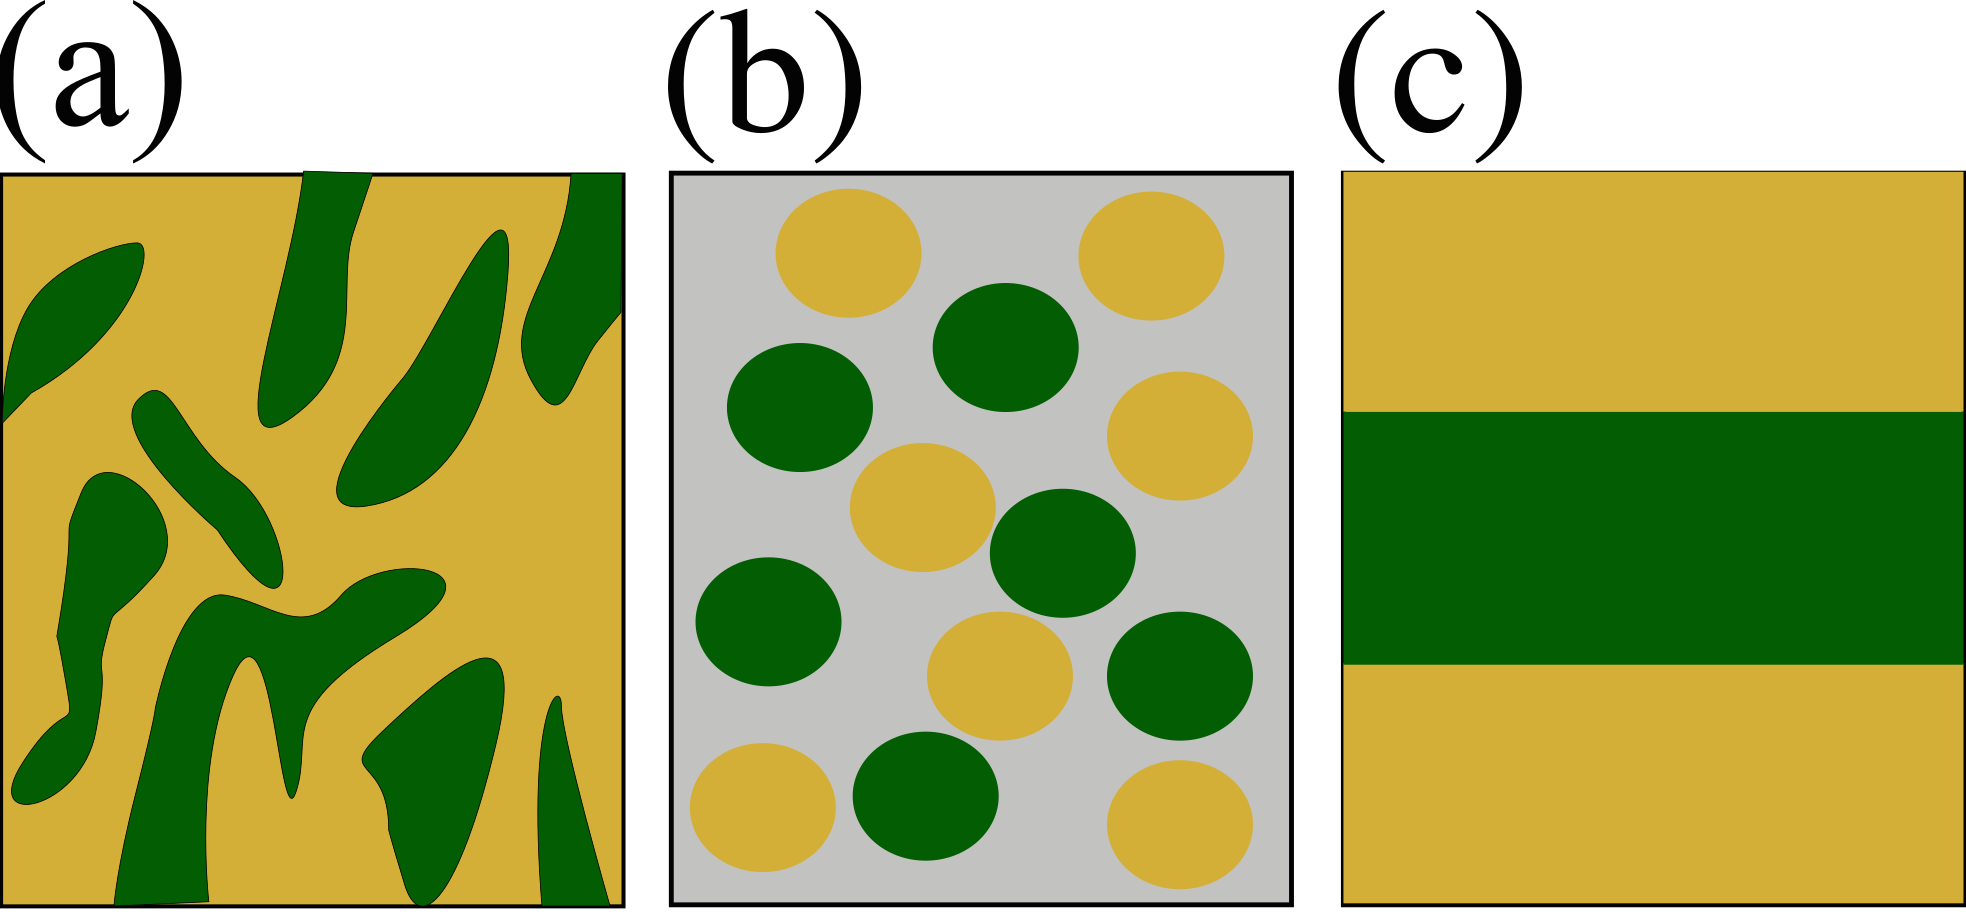
\includegraphics{mgo/image1.png}
\end{figure}

\begin{figure}[h]
\caption{
Dependence of the intensity of the 111 Bragg peak of
MgO as a function of occupancies of the 2p orbitals of Mg2+ and O2-,
according to an atomic form factor (AFF) based model of ionization. This
ratio reaches a maximum factor of 9.6 times the unperturbed value at
full ionization of the O 2p electrons.
}
\centering
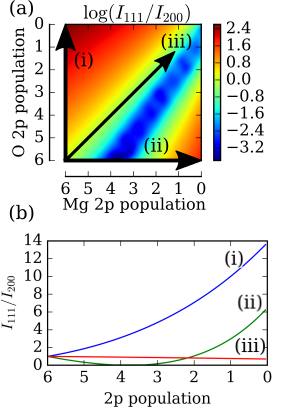
\includegraphics{mgo/image2.png}
\end{figure}

\begin{figure}[h]
\caption{
Electronic temperature evolution during an XFEL pulse
simulated by the radiative collisional code SCFLY. The incident XFEL
photon energy and flux density are 9 keV and 2 x 10\textsuperscript{4}
J/cm\textsuperscript{2}, respectively. The dashed line represents the
temporal profile of the incident XFEL pulse.
}
\centering
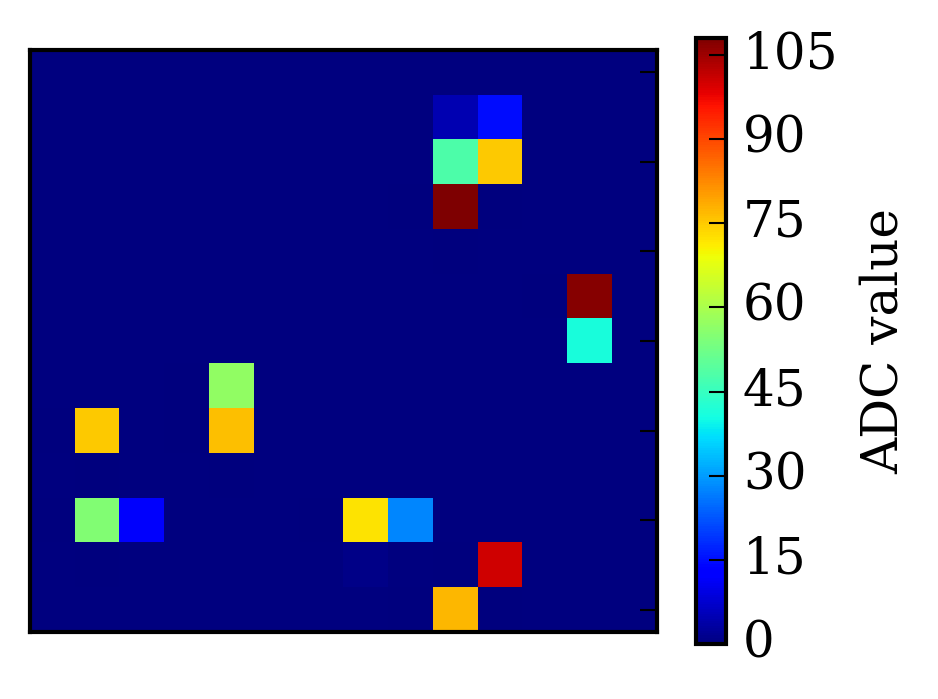
\includegraphics{mgo/image3.png}
\end{figure}

\begin{figure}[h]
\caption{
Evolution of the mean charge states Mg and O of during
an XFEL pulse simulated by the radiative collisional code SCFLY. The
incident XFEL photon energy and flux density are 9 keV and 2 x
10\textsuperscript{4} J/cm\textsuperscript{2}, respectively. The dashed
line represents the temporal profile of the incident XFEL pulse.
}
\centering
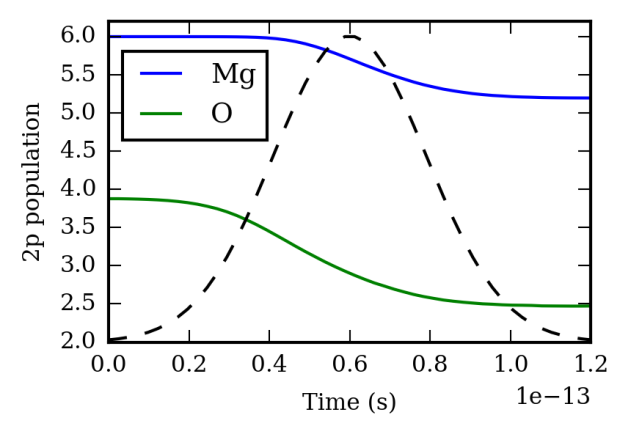
\includegraphics{mgo/image4.png}
\end{figure}
